
\subsection{GDELT Dataset}

\subsubsection{Sparsity in GDELT}

The space of news events spanned by all columns in GDELT is much larger than the subspace we expect news to lie on. There are likely to be at least two modes of low-dimensional interactions in the data: (1) that actors only interact within small cliques and (2) that each actor is involved in a small set of events. We conducted an initial analysis on a random sample of days before August 2015 to avoid making conclusions that overfit the test data.

\begin{figure}[ht]
\vskip 0.2in
\begin{center}
\centerline{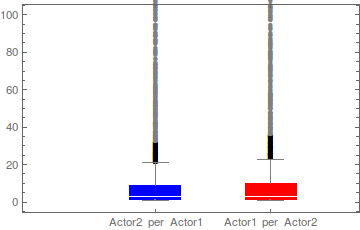
\includegraphics[width=\columnwidth]{images/actors-per-actor.png}}
\caption{Box-and-whisker plot of number of distinct actors each CAMEO actor interacts with (each event may have up to 2 involved actors, where the first inflicts the action), performed on the day-stratified random sample of the events. The medium number of co-actors for both Actor1 and Actor2 categories is 3, with a Q3 of 9 and 10 and maximum of 988 and 990, respectively. The sample contained about 124K events total. The outliers with many interactions are generic or common names, such as \texttt{PRESIDENT} or \texttt{UNITED STATES}.
}
\end{center}
\vskip -0.2in
\label{fig:actors-per-actor}
\end{figure} 

As Figure \ref{fig:actors-per-actor} demonstrates, actor count is a heavily skewed distribution. This gives us confidence that actors are indeed in small cliques for the sampled days. We conduct a similar inspection for the number of unique CAMEO coded events per actor in Figure \ref{fig:events-per-actor}:

\begin{figure}[ht]
\vskip 0.2in
\begin{center}
\centerline{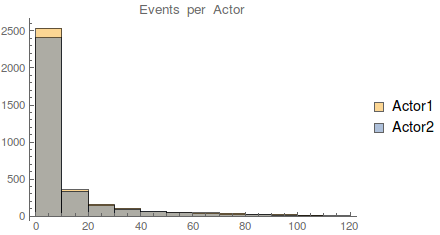
\includegraphics[width=\columnwidth]{images/events-per-actor}}
\caption{Number of events that occur for individual actors. The median actor encounters 3 events, and the 75\% most active ones still see less than 15. This diagram only shows the 95\% least active actors.}
\end{center}
\vskip -0.2in
\label{fig:events-per-actor}
\end{figure} 

Because of the sparsity that is present, we wish to reduce the dimension of our data, which originally consists of over 300 million points in $\mathbb{R^{58}}$ for three reasons: 1) to more accurately represent it, 2) so we can generate models in a continuous space of reduced-dimension tuples of real values (instead of having some categorical values), and 3) so our data pipeline only has to handle a reduced data size.

We found that classical dimensionality reduction was not tractable to apply to a dataset of this size - the highly categorical nature of the dataset results in a large dimensional expansion when preparing numeric inputs to the algorithms. Because of this, and because of our dataset's observed sparsity, we turned to a clustering based approach. 

%\subsection{Bloomberg Commodity Prices}
%up and down spikes
%normally distributed about 0